\documentclass[twocolumn]{emulateapj}
\usepackage{graphicx}

\usepackage{float}
\usepackage[pdftex,
            bookmarks=true,
            breaklinks,
            pagebackref=true]{hyperref}         
            
\usepackage{multirow}

\usepackage{savesym}
\savesymbol{tablenum}
\usepackage{siunitx}
\restoresymbol{SIX}{tablenum}

% \columnwidth = 245.26653 pt = 3.39 in
% \textwidth = 513.11743 pt = 7.10 in

\shorttitle{Modal Noise Minimization}
\shortauthors{Petersburg et al.}

\begin{document}

\title{Modal Noise Mitigation through Fiber Agitation for Fiber-fed Radial Velocity Spectrographs}

\author{Ryan Petersburg, Tyler McCracken, Dominic Eggerman, Colby Jurgenson, David Sawyer, Debra Fischer}
\affil{Department of Astronomy, Yale University, 52 Hillhouse Ave, New Haven, CT 06511, USA; ryan.petersburg@yale.edu}

\begin{abstract}

Optical fiber modal noise is a critically limiting factor for high precision spectroscopy signal-to-noise in the near-infrared and visible. Unabated, especially for highly coherent light sources, modal noise can induce radial velocity errors that hinder the discovery of low-mass (and potentially earth-like) planets. Previous research in this field has found sufficient modal noise mitigation through use of an integrating sphere, but this requires extremely bright light sources, a luxury not necessarily afforded calibration for the next-generation of high resolution optical-range spectrographs. Otherwise, mechanical agitation, which ``mixes'' the fiber's modal patterns and allows the noise to be averaged over minutes-long exposures, provides some noise reduction but the methods have not been fully optimized by the community. Therefore, we have filled out the parameter space of modal noise agitation techniques in order to better understand agitation's contribution to mitigating modal noise and to discover the optimal strategy for agitating fibers. We found that modal noise was best suppressed by the chaotic nature of coupled harmonic motion at high amplitude for fibers with large core diameters and low azimuthal symmetry, reducing modal noise induced radial velocity error to below 10 cm/s. This work has subsequently influenced the design of a fiber agitator to be installed with the Extreme Precision Spectrograph.

\end{abstract}


\section{Introduction}
\label{sec:intro}

The radial velocity (RV) method for exoplanet detection continues to push towards the goal of \SI{10}{\centi\meter\per\second} precision that is necessary for the discovery of earth-like planets orbiting G and K stars in their respective habitable zone \citep{Fischer2016}. The next-generation of RV spectrographs operating in the optical including but not limited to those such as the Extreme Precision Spectrograph \citep[EXPRES,][]{Jurgenson2016}, ESPRESSO \citet{Megevand2012}, NEID \cite{}, the Keck Planet Finder\cite{} and others, require precision engineering and extreme stability to yield such results.
% there is also MaroonX, CARMENES, the Planet Finding Spectrograph, a whole ton, not sure if they all require mentioning but people get their feathers ruffled.

Fiber coupling the spectrograph to the telescope has become an essential and standard method for planet hunting spectrographs enabling the spectrograph itself to be located in an controlled environment, isolating it from vibrational and thermal noise. Linking the telescope to the spectrograph via fiber also leverages the spatial scrambling properties inherent to fibers that, for the most part, decouple the variations on the input from the output producing a stable illumination of the spectrograph optics\citep{Hunter1992}. This effect has been amplified through the use of double scramblers \citep{Halverson2015a, Spronck2015} and non-circular fiber geometries including octagonal and rectangular fibers\citep{Chazelas2010, SPronck2012, Plavchan2013}.

Optical fibers also transmit light from calibration sources--such as wavelength calibrators and broadband flat-field sources--into the spectrograph. Laser frequency combs, specifically the more appropriate Astrocomb \citep{Probst2014} recently deployed at HARPS and soon to be with EXPRES, produce thousands of ultra narrow, evenly spaced emission lines over a wide frequency range. When these highly coherent lines propagate through a multi-mode fiber, they create a source of noise that limits the signal-to-noise ratio (SNR) of the instrument and potentially induces false signals into the data. This noise is caused by interference between the finite number of electromagnetic modes that can propagate along a multi-mode fiber.%and has therefore been coined \textit{modal noise}.

% This paragraph will need some work. It is tough to not step in it here but this should be mentioned.
Some next-generation RV spectrographs \citep[e.g. iLocater,][]{Crepp2016} have moved to a completely single-mode fiber architecture to help alleviate these complications. As apparent in their name, single-mode fibers only propagate a single electromagnetic mode and are therefore free from any modal noise. Due to the small core-size of single-mode fibers, however, coupling light from the telescope into these fibers is challenging, requiring robust adaptive optics that have not yet been fully developed. Additionally, single-mode fibers have a very limited bandwidth over which they propagate a single-mode. Therefore, these fibers may not be truly single-mode across the full band of wavelength calibration meaning the optical design requires multiple band-depend paths. Finally, \citet{Halverson2015b} asserts that a type of polarization ``modal noise'' exists in single mode fibers. Thus, the study of modal noise reduction methods may still be necessary even for these novel single-mode-fiber injected instruments.

In this paper, we attempt to discern the optimal strategy for reducing modal noise in multi-mode fibers propagating coherent visible light through mechanical agitation. We begin by defining modal noise and exploring how previous experiments have mitigated it through static and dynamic methods (section \ref{sec:modal_noise_intro}). We then describe our own methods of fiber agitation (section \ref{sec:experimental_setup}) and discuss results from using these methods on fibers of varying cross-sectional shapes and coupling permutations (section \ref{sec:results}). Finally, we relate these results to limits in RV precision (section \ref{sec:rv_precision}) and discuss how these results should be applied to next-generation RV spectrographs (section \ref{sec:conclusions}). The work in this paper was conducted to influence design decisions for EXPRES.

\section{Optical Fiber Modal Noise}
\label{sec:modal_noise_intro}

Light propagates through an optical fiber in an integer number of electromagnetic modes. The exact calculation for this value is non-trivial since it depends on the instantaneous fiber geometry, injection parameters, and many other variables. The maximum number of modes for a step-index circular cross-section fiber is approximately given by
\begin{equation}
M_{circ} \approx \frac{4}{\pi ^2} V^2
\label{eq:max_modes}
\end{equation}
where $V$ is the normalized frequency of the fiber given as
\begin{equation}
V = \Bigg( \frac{2 \pi r \mathrm{NA}}{\lambda} \Bigg) ^2 .
\label{eq:norm_freq}
\end{equation}
$\mathrm{NA} = \sqrt{n_{core}^2 - n_{clad}^2}$ is the numerical aperture of the fiber determined by the core ($n_{core}$) and cladding ($n_{clad}$) indices of refraction, $r$ is the core radius, and $\lambda$ is the wavelength of propagated light. This approximation is more difficult for a rectangular fiber, but \citet{Nikitin2011} shows empirically using electromagnetic and geometrical arguments that
\begin{equation}
\frac{M_{rect}}{M_{circ}} \propto \frac{ab}{r^2}
\label{eq:prop_modes}
\end{equation}
where $a$ and $b$ are the side lengths of the rectangular cross-section. Therefore, we will assert more generally that
\begin{equation}
M \propto A \Bigg( \frac{\mathrm{NA}}{\lambda} \Bigg) ^2
\label{eq:mode_area}
\end{equation}
where $A$ is the cross-sectional area of the fiber regardless of shape.

%This result is presented without a leading coefficient (that may depend on fiber shape) because it is not rigorously derived or experimentally validated; however, this relationship is extremely useful

\begin{figure}
\centering
	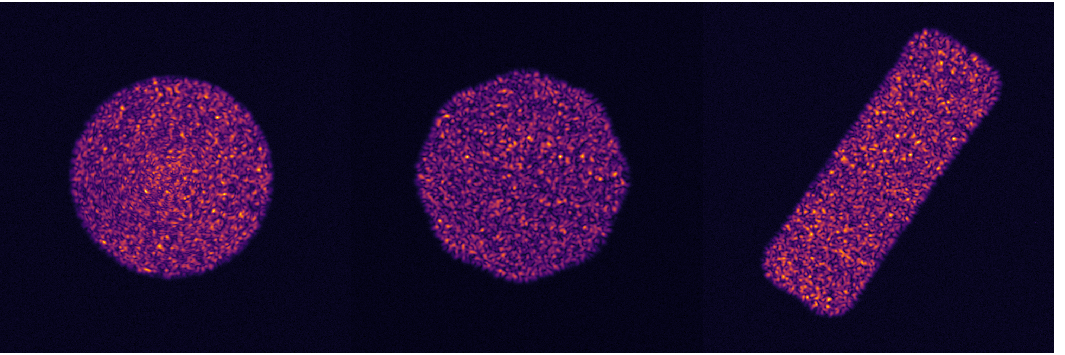
\includegraphics[width=\columnwidth]{images/fiber_example.pdf}
	\caption{Examples of unmitigated modal noise for a rectangular (left), octagonal (middle), and circular (right) optical fiber. All three fibers shown here have approximately the same cross-sectional area, meaning that they each are propagating about the same number of electromagnetic modes (see section \ref{sec:experimental_setup}). Brightness in this image is scaled by the square root of photon count to emphasize the speckles.}
\label{fig:fiber_example}
\end{figure}

When coherent light is propagated through a multi-mode fiber, a high contrast speckle pattern known as modal noise is produced at the output for both the near-field (fiber face) and far-field, figure \ref{fig:fiber_example}. Modal noise is an inherent property of all multi-mode fibers regardless of the cross-sectional core shape \citep{Sablowski2015}. It arises from light coupling from mode-to-mode as it propagates through fiber, resulting in slight variances in the path length traveled and producing the observed interference or speckle pattern. For RV spectrographs this causes two problems: 1) it limits the maximum signal-to-noise ratio and 2) systematic variations in the speckle pattern will mask themselves as minute shifts on the focal plane causing errant RV signatures.

\subsection{Limit on SNR}

Due to its high contrast, modal noise can severely decrease the signal-to-noise ratio of an RV spectrograph \citep{Epworth1978, Baudrand2001, Lemke2011}. Additionally, if the speckle pattern drifts between exposures, especially with some period of motion, modal noise can cause errant RV signatures in the data that is distinct from errors due to poor scrambling \citep{Mahadevan2014}.

Modal noise's dependence on static physical properties of optical fibers is well documented and follows from theory. Modal noise SNR is increased for larger fiber core diameters as in equation \ref{eq:max_modes} \citep{Sablowski2015, Lemke2010} and for non-circular fibers over circular fibers \citep{Sturmer2016, Sablowski2015}. Increasing the number of static bends in a fiber slightly increases SNR \citep{Imai1979}. Far field modal noise SNR is strongly anti-correlated with injected focal ratio \citep{Sablowski2015}, while the near field modal noise SNR is independent of injected focal ratio \citep{Baudrand2001}. Finally, modal noise SNR was shown to be anti-correlated with wavelength (as expected by equation \ref{eq:max_modes}), poorly responsive to input pupil obstructions, and independent of fiber length greater than a few meters \citep{Baudrand2001}.

\subsection{Dynamic variations}

Modal noise is also affected by dynamic optical properties, meaning it can induce false RV's on the spectrograph, in addition to being an issue of SNR. The speckle pattern is heavily wavelength dependent as seen in equation \ref{eq:mode_area}. However, next-generation RV spectrographs are using stable wavelength calibrators rendering this problem effectively irrelevant. Otherwise, the speckle pattern seen at the end of a fiber shifts over time due to many reasons, but most commonly because of \citep{Epworth1978}:
\begin{enumerate}
\item Temperature variation
\item Fiber input illumination variation
\item Fiber movement (bending, twisting, etc.)
\end{enumerate}
These three conditions inevitably pose problems when imaging a spectrum since they are inherent to modern fiber-fed RV spectrographs \citep{Baudrand2001, Mahadevan2014}. There is typically a temperature difference between the telescope and the spectrograph, fluctuations in atmospheric density change the fiber illumination, and the telescope slowly slews throughout the night.

%It is important to note here that \citet{Epworth1978} also includes spatial filtering as a requirement for complications from modal noise. Spatial filtering is historically assumed since many RV experiments use rectangular slits over circular fibers when injecting light into the spectrograph optics. However, as shown in section \ref{sec:rv_precision}, modal noise is still a detriment to RV precision even for an unfiltered rectangular fiber, therefore the spatial filter requirement has been removed.

Modal noise can be reduced by continuously exacerbating one of the above three causes of drift, thereby shifting the speckle pattern throughout an appropriately long camera exposure and averaging out the noise. Controlled temperature variation (option 1) is non-ideal because a 1 meter fiber requires approximately $8 ^\circ \mathrm{C}$ fluctuations to visibly decorrelate the speckle pattern \citep{Redding2013}, a temperature change much too large to guarantee optomechanical stability. Therefore, RV spectrographs have been left with either varying the illumination (option 2) or shaking the fiber (option 3).

\begin{table*}
\centering
\caption{Previous study of dynamic modal noise mitigation methods}
	\begin{tabular}{cccc}
		\hline
		Reference & Method & Frequency & Amplitude \\
		\hline\hline
		\citet{Daino1980} & Loudspeaker & 110 Hz & ``Sufficient'' \\
		\hline
		\citet{Baudrand2001} & --- & 30 Hz & 1 mm \\
		\hline
		\multirow{2}{*}{\citet{Lemke2011}} & Loudspeaker & 1.5 Hz & --- \\
		 & Loudspeaker & 80 Hz & --- \\
		\hline
		\multirow{3}{*}{\citet{McCoy2012}} & Paint mixer & 60 Hz & --- \\
		 & Hand agitated & 1-2 Hz & 10-15 cm \\
		 & Mechanical agitator & ``Low'' & ``High''\\
		\hline
		\multirow{2}{*}{\citet{Plavchan2013}} & ``Tweeter'' & 100 Hz & 1 mm \\
		 & ``Woofer'' & 1 Hz & 25 mm \\
		\hline
		\multirow{3}{*}{\citet{Mahadevan2014}} & Int. Sph. + Diff. & --- & ---\\
		 & McCoy agitator & ``Low'' & ``High' \\
		 & Hand agitation & 1-2 Hz & 10 cm \\
		\hline
		\multirow{2}{*}{\citet{Halverson2014}} & Int. Sph. + Diff. & --- & --- \\
		 & Int. Sph. + OAP & --- & --- \\
		\hline		
		\citet{Roy2014} & Rail agitator & ``Low'' & ``High'' \\
		\hline
		\citet{Sablowski2015} & Mechanical ``Excenter''& 2 Hz & 20 cm \\
		\hline
	\end{tabular}
\label{table:previous_studies}
\end{table*}

As summarized in table \ref{table:previous_studies}, various modal noise reduction techniques have been previously explored. The majority deal with some form of agitation that physically changes the position of the fiber (mechanical agitation) while \citet{Mahadevan2014} and \citet{Halverson2014} explored the effectiveness of varying the illumination of the fiber face. The variation in frequency and amplitude for the mechanical agitation methods is unfortunately quite wide and connections are difficult to make. However, there have been slight trends in the results and the discussed assumptions so far are as follows:
\begin{itemize}
\item The frequency of agitation should be greater than $1/\tau$, where $\tau$ is the exposure time \citep{Baudrand2001}
\item Noise is more effectively reduced by high amplitude motion \citep{Lemke2011, McCoy2012}
\item Higher frequencies (with an upper limit) show further noise reduction \citep{Lemke2011}
\item Adding a high frequency ``tweeter'' to a large amplitude ``woofer'' reduces noise further \citep{Plavchan2013}
\item Hand agitation is better than any form of mechanical agitation \citep{Lemke2011, McCoy2012, Mahadevan2014, Roy2014}
\end{itemize}
Although this has been good for subjective intuition, the exact mechanisms behind the improvements in SNR and prevention of RV drift have not been explored.

Varying the input illumination of a fiber using an integrating sphere, diffuser, and rotating mirror showed gradual improvements in modal noise reduction due to the addition of further illumination variation. However, the integrating sphere, an integral part of these methods, has a throughput efficiency of approximately $10^{-6}$ and is not feasible to be introduced in the science light optical path. To allow flexible observing programs, particullary science observations bracketed by precision wavelength calibration sources, the modal noise mitigation technique needs to be efficient

In the following sections, we fill out the parameter space of fiber agitation methods to a greater extent than previous studies. We are interested in seeing trends across different amplitudes, frequencies, fiber shapes/sizes, and coupling permutations to make more precise conclusions about the nature of modal noise mitigation through fiber agitation.

\section{Experimental Setup}
\label{sec:experimental_setup}

The number of modes a fiber supports is largely determined by its cross-sectional area. We first explored the effect of fiber size on modal noise using mechanical agiation. Larger core fibers support a higher number of modes and it is widely accepted these average over the speckle pattern better than smaller core fibers. The second test was to explore fiber geometry, for this we chose a set of fibers with similar cross-sectional areas. Table \ref{table:fibers} lists the fibers used in our experiments, we explore the fiber size category using circular and octagonal fibers then chareterized the geometry category across circular, octagonal, and rectangular fibers. Notice that the \SI{200}{\micro\meter} circular, \SI{200}{\micro\meter} octagonal, and \SI{100x300}{\micro\meter} rectangular fiber all have approximately the same cross-sectional area, meaning they can each support a similar number of modes.

\begin{table}
\centering
\caption{Tested optical fibers. All fibers have $\mathrm{NA} = 0.22$.}
	\begin{tabular}{ccc}
	\hline
	Shape & Size & Manufacturer \\
	\hline
	\hline
	Circular & \SI{100}{\micro\meter} & Polymicro \\
	Circular & \SI{200}{\micro\meter} & Polymicro \\
	Circular & \SI{600}{\micro\meter} & Thorlabs \\
	Octagonal & \SI{100}{\micro\meter} & CeramOptec \\
	Octagonal & \SI{200}{\micro\meter} & CeramOptec \\
	Rectangular & \SI{100x300}{\micro\meter} & CeramOptec \\
	\hline
	\end{tabular}
\label{table:fibers}
\end{table}

\begin{figure}
\centering
	\includegraphics[width=\columnwidth]{images/agitators_labelled.png}
	\caption{Linear and circular agitator used in these modal noise tests. The linear agitator rotates along the length of the fiber while the circular agitator rotates perpendicular to it. A small counterweight is present to keep a minimal amount of tension in the fiber and prevent it  from over-bending or bunching up.}
\label{fig:agitators}
\end{figure}

Two different methods of mechanical agitation are used: the first produces a linear type motion in which the fiber is moved up and down, the other is a circular type motion in which the fiber is rotated perpendicular to direction of propagation. The linear agitation has variable amplitude allowing for 80-\SI{320}{\milli\meter} agitation amplitudes at \SI{80}{\milli\meter} intervals and a variable frequency in the range of 0.03 to \SI{1.0}{\hertz}. For the circular agitator, the fiber is rotated in circular path with a set amplitude of \SI{80}{\milli\meter} at a variable frequency of 0.1 to \SI{1.5}{\hertz}. Routing a fiber through both agitators produces what we call ``coupled agitation''.  Both agitators are shown in figure \ref{fig:agitators}, frequencies are independently set by adjusting the appropriate DC-motor drive voltage. The amplitude of the linear agitator is set by the position of the lifting arm and a small counterweight is present to keep a minimal amount of tension in the fiber between the agitators and prevent it from folding on itself.

\begin{figure}
\centering
	\includegraphics[width=0.5\columnwidth]{images/tweeter.jpg}
	\caption{PASCO Scientific economy wave driver used to test high-frequency, low-amplitude agitation (tweeter). \url{https://www.pasco.com/images/products/wa/WA9854_MAIN_171382.jpg}}
\label{fig:tweeter}
\end{figure}

To test high-frequency, low-amplitude agitation, we use a PASCO Scientific ``Economy Wave Driver'' shown in figure \ref{fig:tweeter}. This device, attached to a sine wave function generator, produces approximately \SI{5}{\milli\meter} amplitude for 10-\SI{30}{\hertz} oscillations. It can be driven at higher frequencies, but the amplitude would not be large enough to produce significant fiber motion.

All image data was collected with the Fiber Characterization Station (FCS, figure \ref{fig:fcs}), a multipurpose device that is able to simultaneously image the input face, output face (or near field), and output pupil (or far field) of the fiber under test. Specifications for the FCS cameras are listed in table \ref{table:cameras}.

\begin{figure}
\centering
	\includegraphics[width=\columnwidth]{images/fcs_schematic.png}
	\caption{Schematic of the Fiber Characterization Station. Light from either a single-mode fiber-fed \SI{652}{\nano\meter} Toptica diode laser or from a selection of Thorlabs mounted LEDs fed by a \SI{100}{\micro\meter} circular fiber is fed into the station in the bottom left. This light is spatially filtered, collimated, and injected into the test fiber. The injection face of the test fiber is imaged at 10x magnification by the input camera to allow for precision alignment. Light propagates through the test fiber and our choice of agitator mixes the modes. Light is then ejected from the test fiber and split between the 10x magnified near field camera and the far field camera.}
\label{fig:fcs}
\end{figure}

\begin{table}
\centering
\caption{Fiber Characterization Station imaging specifications}
	\begin{tabular}{cccccc}
	\hline
	Name & Camera & Pixel Size & Magnification \\
	\hline \hline
	Input & Atik 450 & \SI{3.45}{\micro\meter} & 10 \\
	\hline
	Near Field & Atik 450 & \SI{3.45}{\micro\meter} & 10 \\
	\hline
	Far Field & Atik 383L+ & \SI{5.4}{\micro\meter} & N/A \\
	\hline	
	\end{tabular}
\label{table:cameras}
\end{table}

Images exposure times are set according to the frequency of agitation such that each exposure lasts exactly one period of rotation. For example, if an agitator is set to rotate at \SI{0.5}{\hertz}, each image will be exposed for \SI{2}{\second}. We do this to confirm that only one full rotation is being recorded and allow for ``number of rotations'' to be another parameter for exploration.

%For each data set, we take a sequence of ten exposures in order to:
%\begin{enumerate}
%\item reduce statistical errors in our SNR calculations potentially caused by camera noise or small problems with our agitators
%\item observe the effects of agitation at longer exposures time by co-adding multiple single-rotation images together. 
%\end{enumerate}
%Whenever collecting images sets to be compared, we also take a set of images with the agitator turned off (hereafter called \textit{unagitated images}) and a set of images using a broadband LED light source. This allows for direct comparison to a worst-case and best-case scenario respectively.

Each data set is comprised of a 10 exposures each of the following cases:
\begin{enumerate}
\item the fiber being actively agitated
\item the fiber routed through the agitator but without agitation
\item the unagitated fiber illuminated with a broadband LED.
\end{enumerate}
Multiple images are taken to reduce statistical errors in our SNR calculations potentially caused by camera noise or small problems with our agitators and to observe the effects of agitation at longer exposures time by co-adding multiple single-rotation images together. The LED source acts as a best-case scenario and the unagitated as a worst case.

We quantify modal noise using the SNR of light within the fiber face of the near field image calculated as
\begin{equation}
\mathrm{SNR} = \frac{\mathrm{median}(I_{filt})}{\mathrm{stdev}(I_0 - I_{filt})}
\label{eq:snr}
\end{equation}
where $I_0$, the original raw image, is heavily median filtered to produce $I_{filt}$. The typical SNR (where the ``signal'' is assumed to be a top-hat function across the fiber face) could not be used due to slight intensity-varying diffraction effects across the near field image. Subtracting $I_{filt}$ from $I_0$ therefore produces a noise pattern that reflects the modal noise and not these large-scale diffraction-caused variances. We use a circular 51-pixel median filter rather than a low-order polynomial or Gaussian fit because these functions could not sufficiently fit the raw fiber images. The size of the filter kernel was chosen such that speckles on unagitated images were sufficiently filtered without removing structure from the edges of the fibers. The numerator in equation \ref{eq:snr} is calculated as the median (rather than the mean, for example) of $I_{filt}$ to prevent dust on the fiber face or optics from skewing this value.

We calculate the SNR for each individual image and average them together within each data set to yield a single-rotation SNR. We then co-add images 1-2, 1-3, 1-4, ..., 1-10 and calculate the SNR for each case. The SNR for images 1-10 is presented as the ten-rotation SNR and each intermediate step as two-rotation SNR, three-rotation SNR, etc.

Far field images are taken for each data set and analyzed using the maximum intensity rather than the median intensity as the numerator in equation \ref{eq:snr}. The far field speckle pattern is of interest in precision RV spectroscopy as it is what illuminates the optics. However, mapping the far field speckle pattern to RV error would require numerical simulations with the optical design software and  is out of the scope of this paper. That being said, all results listed in the following section may be extended to the far field though we omit this data for conciseness.

\section{Results}
\label{sec:results}

\subsection{Method of Agitation and Fiber Geometry}
\label{subsec:ag_snr}

\begin{figure}
\centering
	\includegraphics[width=\columnwidth]{images/ag_snr.pdf}
	\caption{SNR comparison for varying fiber geometries and agitation methods. SNR for 10 rotation images was calculated after co-adding ten single rotation images.}
\label{fig:ag_snr}
\end{figure}

We compare the two individual agitation methods and coupled agitation using all of the fibers previously listed in table \ref{table:fibers}. The linear agitator was set to an amplitude of \SI{80}{\milli\meter} and the frequency of both agitators to \SI{1.0}{\hertz}, all images are taken with \SI{1}{\second} exposures.

Results for the single-rotation and ten-rotation cases are shown in figure \ref{fig:ag_snr}. Across all fiber shapes and sizes and number of rotations, the linear agitator appears to be slightly better than the circular agitator. There is a similar increase in SNR when looking at coupled agitation in single-rotations. However, coupling the agitation over ten-rotations significantly increases the SNR for all fiber configurations.

\begin{figure}
\centering
	\includegraphics[width=\columnwidth]{images/fiber_improved.pdf}
	\caption{Ten-rotation, coupled agitation images using the same three fibers shown in figure \ref{fig:fiber_example}.  The diffraction pattern is clearly seen, but otherwise, the presence of speckles in these images is significantly diminished. With larger amplitude in both the circular and linear agitator, the SNR will continue to improve. These images were taken as part of the data in section \ref{subsec:ag_snr}.}
\label{fig:fiber_improved}
\end{figure}

Ten-rotation images of the three larger fibers using the coupled agitation method are shown in figure \ref{fig:fiber_improved}. Compared to those shown in figure \ref{fig:fiber_example}, the speckle patterns when using coupled agitation are nearly non-existent.

\begin{figure}
\centering
	\includegraphics[width=\columnwidth]{images/rect_snr_vs_time.pdf}
	\caption{SNR for the 100x\SI{300}{\micro\meter} rectangular fiber using various agitation methods. The SNR is calculated after co-adding the 1 rotation images.}
\label{fig:rect_snr_vs_time}
\end{figure}

To better understand why coupled agitation is so effective at reducing modal noise at longer exposures, we also analyze the effect of each agitation method over multiple rotations, as shown in figure \ref{fig:rect_snr_vs_time} for the \SI{100x300}{\micro\meter} rectangular fiber. SNR shows continued improvement beyond a single rotation when coupling the agitation methods at a similar rate to when the fiber is lit by an LED, a broadband source. Circular and linear agitation, however, are effectively plateaued after the first rotation.

\subsection{Adding a Tweeter}

\begin{figure}
\centering
	\includegraphics[width=\columnwidth]{images/tweeter_snr.pdf}
	\caption{SNR comparison when adding a tweeter to the coupled agitation method for a rectangular fiber. Exposure times are set to \SI{2.0}{\second}, approximately the period of one rotation for the coupled agitator, and the tweeter is set to \SI{20}{\hertz}.}
\label{fig:tweeter_snr}
\end{figure}

We also test the high-frequency, low-amplitude tweeter proposed by \citep{Plavchan2013} in tandem with our coupled agitation to see if it supplies significant improvement to modal noise SNR. We set the linear agitator to \SI{240}{\milli\meter} and \SI{0.5}{\hertz} and the circular agitator to approximately the same frequency. All exposure times are set to \SI{2.0}{\second}.

The results are shown in figure \ref{fig:tweeter_snr}. The tweeter improves SNR above coupled agitation alone regardless of exposure time. However, the magnitude of this improvement is minimal and is far outweighed by the improvement due to coupled agitation.

\begin{figure*}[t]
\centering
	\includegraphics[width=\textwidth]{images/amp_freq_snr.pdf}
	\caption{SNR comparison for varying amplitudes using the linear agitator (left) and varying frequencies using each of the linear (center) and circular (right) agitators. For the amplitude tests, the linear agitator was set at \SI{0.5}{\hertz}. For the linear agitator frequency test, the amplitude was set to \SI{240}{\milli\meter}. The circular agitator can only be set to an amplitude of \SI{80}{\milli\meter}. Integration times were set to match the period of 1 rotation (i.e. \SI{2}{\second} for \SI{0.5}{\hertz} agitation). The ``10 rotations'' data was calculated after co-adding 10 of these 1 rotation images. Results in the far field yielded similar correlations between amplitude, frequency, and SNR.}
\label{fig:amp_freq_snr}
\end{figure*}

\subsection{Amplitude and Frequency of Agitation}
\label{subsec:amp_freq}

We use the \SI{100x300}{\micro\meter} rectangular fiber and the two agitators separately to test the effects of agitation amplitude and frequency of rotation on the SNR. We can only test amplitude on the linear agitator and take an image set for each position on the rotating arms. We test frequency on each of the linear and circular agitators at approximately equally spaced frequencies across their entire frequency range.

Results from these tests are shown in figure \ref{fig:amp_freq_snr}. There is a strong position correlation between linear agitation amplitude using both the single-rotation and ten-rotation analyses. There also appears to be a slight increase in SNR for the linear agitator at higher frequencies after ten rotations, however there is no such increase for the single-rotations or any of the frequencies when using the circular agitator.

\subsection{Fiber Coupling}

\begin{table}
\centering
\caption{Fiber assemblies tested for the fiber coupling experiment}
	\begin{tabular}{ccc}
	\hline
	Test & 1st Fiber & 2nd Fiber \\
	\hline \hline
	1 & Circular \SI{200}{\micro\meter} & Circular \SI{200}{\micro\meter} \\
	\hline
	2 & Circular \SI{100}{\micro\meter} & Circular \SI{200}{\micro\meter} \\
	\hline
	3 & Octagonal \SI{200}{\micro\meter} & Circular \SI{200}{\micro\meter} \\
	\hline
	\end{tabular}
\label{table:fiber_coupling}
\end{table}

%Most next-generation RV spectrographs use double-scramblers in their fiber architecture as briefly described in section \ref{sec:intro}. Thus, light is propagated through more than one fiber between the calibration sources, telescope, and spectrograph. To study the effects of such an architecture, we agitate individual fibers in a multi-fiber assembly where each fiber could have different core sizes and shape. The fibers are coupled using a 1:1 ratio, two-lens setup with large enough NA to avoid light loss. We test three distinct cases outlined in table \ref{table:fiber_coupling} and compare them against agitating a single \SI{200}{\micro\meter} circular fiber. The fibers are agitated using the linear agitator at \SI{80}{\milli\meter} and \SI{1.0}{\hertz}. We could not use the circular agitator for these tests since the hole is not large enough to accommodate threading two fibers.

It is not uncommon for RV spectrographs to have multiple fiber links for carrying calibration and/or science light from the source (lamp or telescope respectively) to the spectrograph and ultimately detector. This results in having to couple light from one fiber to another and begs the question, is there a preferred fiber to agitate or must we agitate as many as possible? Agitating the first fiber in a multi-fiber system serves to vary the input illumination of subsequent fibers, similar to the integrating sphere proposed by \citep{Mahadevan2014} and \citep{Halverson2014}. To study the effects of such an architecture, we agitated individual fibers in a multi-fiber assembly where each fiber could have different core sizes and shape. We test three distinct cases outlined in table \ref{table:fiber_coupling} and compare them against agitating a single \SI{200}{\micro\meter} circular fiber. For this test fibers were agitated using the linear agitator at \SI{80}{\milli\meter} and \SI{1.0}{\hertz}.

\begin{figure}
\centering
	\includegraphics[width=\columnwidth]{images/coupled_fibers.pdf}
	\caption{SNR for various arrangements of coupled fibers with varying core diameter and cross-sectional shape. All fibers are assumed to be circular unless otherwise stated on the plot. The SNR for a single \SI{200}{\micro\meter} circular fiber is also presented for both 1 rotation (dashed) and 10 rotations (solid).}
\label{fig:coupled_fibers}
\end{figure}

The results from these tests are shown in figure \ref{fig:coupled_fibers}. For the most part, the SNR for each test hovers around 10, the same level at which the SNR would be for an uncoupled \SI{200}{\micro\meter} fiber. However, the SNR when agitating only the \SI{100}{\micro\meter} fiber is significantly less than 10. The single-rotation images when agitating the second fiber in the 200-\SI{200}{\micro\meter} test also seem to be abnormally low, but this appears to be repaired over longer exposures. Otherwise, the SNR when agitating both the coupled \SI{200}{\micro\meter} octagonal and \SI{200}{\micro\meter} circular fibers simultaneously is significantly improved.

\subsection{Discussion}
\label{subsec:discussion}

%Our results indicate that large amplitude, relatively high frequency, chaotic coupled harmonic agitation for optical fibers that have large core cross-sectional area and low azimuthal symmetry yield the highest signal to noise. This motion needs to be continuous, to avoid build-up of a single fiber configuration speckle pattern, and can be done anywhere along the length of the fiber, allowing for large distance from a stabilized spectrograph.

Our results can be summarized as follows, the highest SNR is attained when a fiber has been put through as many physical configurations as possible over the length of an exposure. This is best accomplished using a coupled agitation setup comprised of, in our case, a linear and circular motion with the highest amplitude possible on each. One could conceive a random or chaotic agitator as a possible implementation. These conclusions are highly reminiscent of the idea that hand-agitation is consistently better than any form of mechanical agitation. Human motions are much less deterministic than a motor resulting in a more chaotic motion. Our combined linear/circular agitator with slightly different oscillation frequency mimics this behavior since it will chaotically reach many fiber configurations over a single calibration exposure of about \SI{10}{\second}. Note that the motion needs to be continuous to avoid build-up of a static speckle pattern within the exposure.

Our results indicate that large amplitude, relatively high frequency, chaotic coupled harmonic agitation for optical fibers that have large core cross-sectional area and low azimuthal symmetry yield the highest signal to noise. We therefore believe that the most important factor when agitating fibers is to place the fiber into as many physical configurations as possible over a single exposure, and can be done anywhere along the length of the fiber, allowing for large distance from a stabilized spectrograph.

%The most important factor when agitating fibers is to place the fiber into as many physical configurations as possible over a single exposure. By \textit{physical configuration} we mean the amount of ways the fiber is physically oriented in space. For example, say we were to grip the fiber at exactly one position along its length. To maximize SNR, we would need to put that one point into as many unique positions in space as possible during a single exposure. If this point is attached to the linear agitator, larger amplitude rotations increase the circumference of the circle this point would trace and, as indicated by figure \ref{fig:amp_freq_snr}, the SNR improves. Coupled agitation simply adds another grip-point along the fiber, exponentially increasing the combined number of spacial positions and clearly improving the SNR as shown in figure \ref{fig:ag_snr}.

We made this conclusion initially from the data present in figure \ref{fig:amp_freq_snr} which shows a much stronger correlation between amplitude and SNR than between frequency and SNR. The data in figures \ref{fig:ag_snr} and \ref{fig:rect_snr_vs_time} provide further evidence that placing the fiber into more physical configurations further increases the SNR.

Our tweeter tests also provide evidence for our conclusion. Even though the high-frequency device is able to place the fiber into many positions over a single exposure, the difference in these configurations is relatively small. Therefore, the speckle pattern is only ``fuzzed'' a little rather than moved throughout the entire fiber face. Adding a tweeter to a large-amplitude agitator does show some small improvements (since extra ``fuzzing'' would naturally increase SNR), but these improvements are significantly overshadowed by simply having large amplitude motion.

%These conclusions are highly reminiscent of the idea that hand-agitation is consistently better than any form of mechanical agitation. Human motions are typically less deterministic than a motor, meaning that a person hand-agitating the fiber would naturally put it into more physical configurations. Our combined linear/circular agitator with slightly different oscillation frequency mimics this behavior since it will chaotically reach many fiber configurations over a single calibration exposure of about \SI{10}{\second}.

We are also able to confirm previous results that show better mitigation of modal noise for fibers with larger cross-sectional areas and less azimuthally symmetry. As seen in figure \ref{fig:ag_snr}, across all agitation methods, the \SI{200}{\micro\meter} fibers fared better than the \SI{100}{\micro\meter} fibers and the rectangular fiber was consistently far better than the others.

It follows that the location of agitation in a fiber architecture should depend primarily on the cross-sectional area of the fiber. Figure \ref{fig:coupled_fibers} shows that SNR is only significantly worsened if the smaller fiber in a system is agitated over the larger one. This is consistent with our previous conclusion that smaller fibers are less effective when mitigating modal noise. Otherwise, our results indicate that agitating more fibers is helpful, especially if they have different core shapes, but not significantly enough to warrant necessitating this in the design.

Moreover, location of agitation along a single fiber does not seem to matter. Coupling two \SI{200}{\micro\meter} fibers with a 1:1 ratio is effectively adding their lengths together. As shown by figure \ref{fig:coupled_fibers}, the location of agitation is irrelevant, especially for ten-rotation exposures. Therefore, the agitator could be placed anywhere along the length of the fiber (preferably far away from the spectrograph) and it will produce the same magnitude effect on modal noise. This conclusion relies on only one test, however, so it will require further study to absolutely confirm.

\section{Radial Velocity Precision}
\label{sec:rv_precision}

\begin{figure*}
\centering
	\includegraphics[width=\textwidth]{images/rv_error.pdf}
	\caption{Centroid drift and resultant RV error for a slowly agitated fiber (top), coupled agitated fiber (middle), and LED illumination (bottom). The red line in each image is the 30-image average of these centroid drifts, effectively yielding the RV error for \SI{30}{second} exposures.}
\label{fig:rv_error}
\end{figure*}

As discussed in section \ref{sec:modal_noise_intro}, optical fiber modal noise is an issue of centroid drift as well as diminished SNR. To observe how the centroid actuall drifts over time, we test our agitation method on the \SI{100x300}{\micro\meter} rectangular fiber over three hundred \SI{1.0}{\second} exposures.

The resultant RV precision ($\sigma_{RV}$) due to a shifting speckle pattern centroid at the end of a fiber is calculated as:
\begin{equation}
\sigma_{RV} \approx \frac{c}{R} \frac{\sigma_d}{D}
\label{eq:rv_error}
\end{equation}
where $c$ is the speed of light in a vacuum, $R$ is the resolution of the spectrograph, $\sigma_d$ is the standard deviation of fiber near field centroid drift in the dispersion direction and $D$ is the slit width (or short-end length of a rectangular fiber). Importantly, $\sigma_{RV}$ is only the RV error \textit{per resolution element} or \textit{per line} from a wavelength calibration source. Averaging over $N$ lines, we can divide $\sigma_{RV}$ by $\sqrt{N}$ to approximate the total RV error. Notice that for EXPRES, a $R=150,000$ spectrograph fed by a \SI{33}{\micro\meter} slit, reaching the \SI{1}{\meter\per\second} RV precision per line stability requires centroiding to \SI{0.0165}{\micro\meter} along the dispersion direction.

We derive equation \ref{eq:rv_error} from the low velocity approximation of the relativistic Doppler effect
\begin{equation}
\frac{\Delta \lambda}{\lambda} = \sqrt{\frac{1 + v/c}{1-v/c}} - 1 \approx \frac{v}{c}
\label{eq:doppler_effect}
\end{equation}
where $\Delta \lambda$ is the measured shift in wavelength at wavelength $\lambda$ on the spectrograph for a star moving at velocity $v$ relative to Earth. The resolution of a spectrograph is
\begin{equation}
R = \frac{\lambda}{\Delta \lambda_R}
\label{eq:resolution}
\end{equation}
where $\Delta \lambda_R$ is the bandpass of a resolution element. Centroid shifts in the near field of the fiber face can be equated to a measured wavelength shift at the focal plane of the spectrograph:
\begin{equation}
\frac{\Delta d}{D} = \frac{\Delta \lambda}{\Delta \lambda_R}.
\label{eq:spx_shift}
\end{equation}

Using equations \ref{eq:doppler_effect}, \ref{eq:resolution}, and \ref{eq:spx_shift} we show that
\begin{equation}
\frac{v}{c} \approx \frac{\Delta \lambda}{\lambda} = \frac{1}{R} \frac{\Delta \lambda}{\Delta \lambda_R} = \frac{1}{R} \frac{\Delta d}{D}.
\end{equation}
If we take the standard deviation of the data from each side of this equation ($v \rightarrow \sigma_{RV}, \Delta d \rightarrow \sigma_d$) and move $c$ to the right side, we get equation \ref{eq:rv_error}.

The idealized agitation method we use to test RV precision includes the circular agitator oscillating at \SI{1.1}{\hertz} and the linear agitation set at \SI{240}{\milli\meter} and \SI{1.0}{\hertz}. Keeping the two agitators at slightly different frequencies means that a larger range of fiber configurations are reached after about \SI{10}{\second}. We compare this idealized method to a broadband light source (low modal noise) and a slowly agitated fiber (high modal noise). For the slow agitation test, we set only the linear agitator at \SI{80}{\milli\meter} and \SI{0.03}{\hertz} meant to mimic the slight motions of the telescope throughout a night.

The results for these tests are shown in figure \ref{fig:rv_error} where the RV error is calculated using equation \ref{eq:rv_error}. The dispersion direction for a rectangular fiber is along the short end, meaning that the diameter $D$ is \SI{100}{\micro\meter}. The resolution of EXPRES is 150,000 for a \SI{33x132}{\micro\meter} rectangular fiber, so we use $R=50,000$ in equation \ref{eq:rv_error} since our test fiber is three times as large in the dispersion direction.

%Notice that the rectangular fiber does show RV error due to modal noise in the dispersion direction. This is contrary to the assumption made by \citet{Epworth1978} where spatial filtering is required for modal noise to affect the RV measurement of a spectrograph.

These results indicate that coupled agitation reduces errors induced by a slowly moving telescope by about three times and are minimized to about \SI{1.11}{\centi\meter\per\second}. This error is the RV error per line in the spectrograph, meaning that the total RV error could be reduced to below \SI{10}{\centi\meter\per\second} with at least 120 lines, a feat easily achievable with modern day laser frequency combs or other precision wavelength calibrators currently being explored and implemented.
%. EXPRES is using a laser frequency comb with approximately \SI{20}{\giga\hertz} line spacing leading to between 200-500 lines per order on the spectrograph. This will reduce the RV error per order to below \SI{8}{\centi\meter\per\second}.

Using our prototype agitation setup in our lab, we were not able to reach the stability of continuum illumination (\SI{26}{\centi\meter\per\second}). However, we are confident that increasing the amplitude of circular motion, increasing the frequency of both agitators, and adding a ``tweeter'' element will continue to push this limit even lower.

\section{Summary and Application}
\label{sec:conclusions}

\begin{figure}
\centering
	\includegraphics[width=\columnwidth]{images/fiber_rv_error.pdf}
	\caption{Comparison of the long-term agitation methods used in section \ref{sec:rv_precision}--slow agitation (left), coupled agitation (middle), LED source (right)--as \SI{10}{\second} exposures. Brightness directly scales with photon count in these images.}
\label{fig:fiber_rv_error}
\end{figure}

We have tested a wide swath of agitation parameter space with the goal of further understanding the mechanism behind fiber agitation as a method for modal noise mitigation. We found that high amplitude, coupled harmonic motion places the fiber into many physical configurations over a short period of time and therefore reduces modal noise extremely efficiently. As shown in figure \ref{fig:fiber_rv_error}, the coupled agitation method reduces the speckle pattern to levels about as good as a fiber propagating a broadband light source. Such modal noise mitigation can be done at integration times on the order of seconds for relatively dim light source, allowing for direct application to precision RV spectrographs.

\begin{figure}
\centering
	\includegraphics[width=\columnwidth]{images/agitator_model.png}
	\caption{Rendering of the proposed fiber agitator for EXPRES. Both the linear and circular agitator have an independent dc motor operated by remote computer control. This agitator will sit on a shelf across the room from the spectograph and will agitate all fibers that enter the spectrograph during stellar and calibration exposures.}
\label{fig:agitator_model}
\end{figure}

As part of the EXPRES fiber architecture, we will be employing the idealized agitation technique detailed in this paper. We will be combining a \SI{160}{\milli\meter} amplitude circular and linear agitator similar to those seen in figure \ref{fig:agitators}, but with greater stability to support an entire reinforced wrap of cables. A rendering of this design is shown in figure \ref{fig:agitator_model}. The two agitators will oscillate at slightly different frequencies at the maximum speed deemed safe for the fibers. We will potentially include a large tweeter attached directly to the cables to add simultaneous high frequency vibrations to the fibers, since it does show marginal improvement to the SNR. This device will agitate all of the fibers that immediately enter the spectrograph, which includes, most importantly, the rectangular science fiber.

We recommend that other precision RV spectrographs consider the results found in this paper when designing their own fiber agitators. Since it only affects the fibers between light sources and the spectrograph, such improved agitation methods can even be added to spectrographs currently taking data to improve SNR and reduce potential false positions. Modal noise is not a problem that should treated lightly, and its mitigation will help usher in the next-generation of RV spectroscopy and aid in the search for Earth-like worlds.

\acknowledgments

We would like to acknowledge NSF Major Research Instrumentation Award AST 1429365, as well as an NSF Advanced Technologies Instrumentation Award AST 1509436. The author would also like to acknowledge Gabor Furesz for assistance with the Fiber Characterization Station design. The Fiber Characterization Station was built with support from the Fund for Astrophysical Research, Inc. Special thanks to Saki Kamon, Kristoffer Acu\~na, and Dominic Eggerman for their data-taking contributions to this project.

\bibliographystyle{aasjournal}  %for bibtex
\bibliography{modal_noise_mitigation} %for bibtex-example

\end{document}